\chapter{Design}
Angelina Scheler \& Christian Pfeiffer

\section{Einleitung}
Eine weitere Aufgabe, die unsere Gruppe übernommen hat, war das Onboarding für die Stundenplan App. Im Onboarding kann der Nutzer gleich zum Start der App seine Einstellungen zu Fakultät, Studiengang, Semester, Vorlesung und Kalendersynchronisation vornehmen. Das Onboarding wird gestartet, wenn noch keine Angaben zu den genannten Einstellungen gemacht wurden.

\begin{itemize}
\item Neues Design
\item besseres Design
\item iOS Design
\end{itemize}


\section{Mockups}
Unsere Design Sachen sind sehr schön!
\subsection{Screen1}
\begin{enumerate}
\item Fakultät (die die Farbe der App bestimmt)
\end{enumerate}

\begin{figure}[ht]
	\centering
  \frame{ 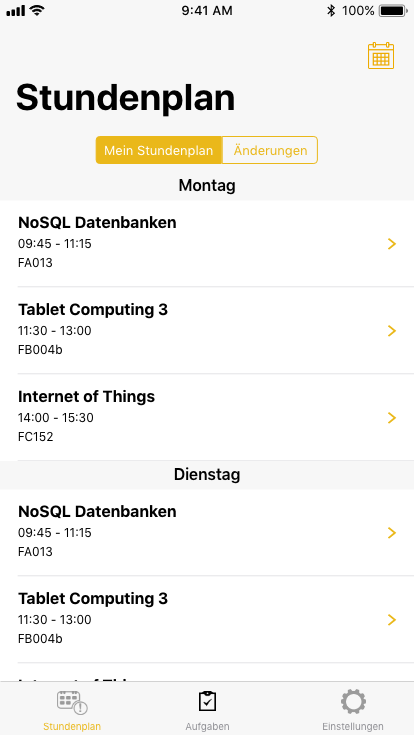
\includegraphics[width=0.9\textwidth]{Mein_Stundenplan} }
	\caption{Mein schönstes Mockup}
	\label{fig1}
\end{figure}